\chapter{Model zur Lösung des CSP-Problems}\label{model}

In diesem Kapitel wird zuerst die Implementierung des Min-Conflicts-Embedder (Abschnitt \ref{minConflictImpl}) mit seinen einzelnen Methoden vorgestellt. Anschließend werden anhand von Klassendiagrammen die Bindungs- (Abschnitt \ref{bindunganforderung}) und Routinganforderungen (Abschnitt \ref{routinganforderung}) näher betrachtet. Dabei wird die innere Struktur betrachtet, die diese Anforderungen hinzufügen, testen und lösen.
\section{Implementierung des Min-Conflicts-Embedder}\label{minConflictImpl}

Die Implementierung des Min-Conflicts-Embedder ist anhand des Aktivitätsdiagramm (Abbildung \ref{fig:minConflictsAkti}) graphisch dargestellt. Zuerst wird die Schleifenvariable der äußeren Schleife mit Null initialisiert und die Methode \textbf{mapTaskRandomly} aufgerufen. In \textbf{mapTaskRandomly} werden alle Tasks einer zufällig gewählten Kachel, die im Programmcode Unit genannt wird, zugewiesen. Es werden dabei Verletzungen der Constraints ignoriert. Anschließend wird der inneren Schleifenvariable k dem Wert Null zugewiesen und die Funktion \textbf{findRandomConflictingTask} aufgerufen. Diese Funktion wählt einen Task aus der Menge C der Tasks aus, die mindestens einen Constraint verletzen. Falls es keinen Task gibt (conflictingTask==null) und somit die Menge C leer ist, wurde eine Lösung gefunden (\textbf{success}). Ansonsten wird überprüft, ob die maximale Anzahl an Schleifendurchgängen (kMax) erreicht wurde. Wenn dies nicht der Fall ist, ruft das Programm die Funktion \textbf{minConflicts} auf. \textbf{minConflicts} bekommt als Parameter den conflictingTask übergeben und versucht für ihn eine geeignete Kachel zu finden, die zu keiner Verletzung eine Bindungs- bzw Routingbedingung führt. Falls es eine derartige Kachel nicht gibt, wird schrittweise der MaxHopConstraint gelockert. Das heißt, dass die Manhattendistanz schrittweise um eins erhöht wird, bis der Algorithmus eine geeignete Kachel gefunden hat. Ist dies der Fall, wird k inkrementiert und die Funktion \textbf{findRandomConflictingTask} wiederum aufgerufen. \\
Hat k den Wert kMax erreicht, so ist der Durchgang beendet und alle Tasks werden ihrer Kachel entzogen (\textbf{unmapTasks}). Die Funktion \textbf{mapTaskRandomly} wird aufgerufen und ein neuer Durchgang beginnt. Falls nach jMax Durchgängen noch keine Lösung gefunden wurde, beendet sich das Programm (\textbf{fail}).

\begin{figure}[H]\centering
  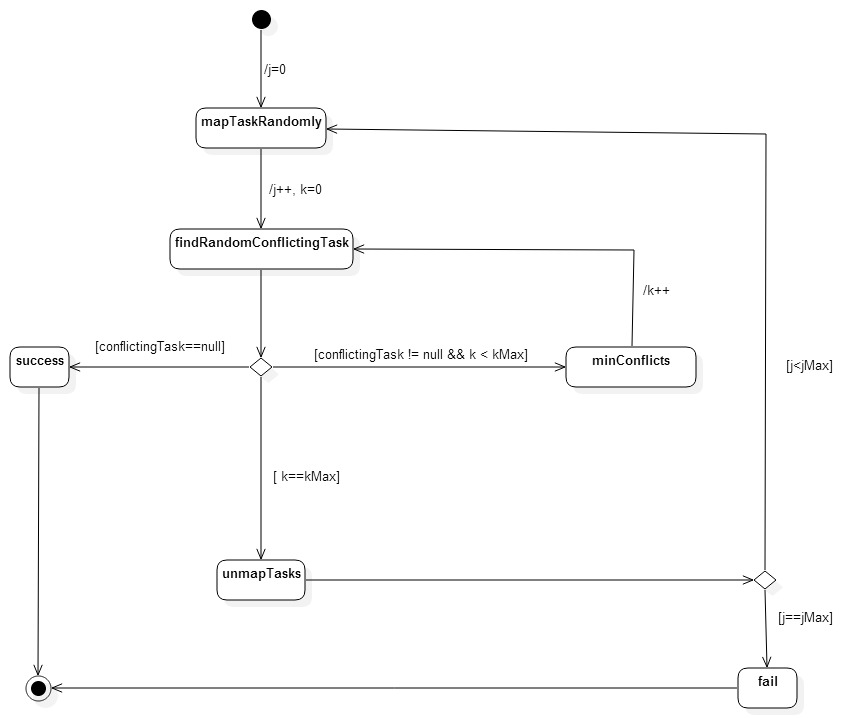
\includegraphics[width = 150mm]{bilder/minAkti.jpg}
  \caption{Das Aktivitätsdiagramm zur Min-Conflicts-Implementierung}\label{fig:minConflictsAkti}
\end{figure}
\section{Klassendiagramm zum Lösen der Bindungs- und Routinganforderungen}


\subsection{Bindungsanforderungen}\label{bindunganforderung}

Die Abbildung \ref{fig:klBind} zeigt das Klassendiagramm zum Lösen von Bindungsanforderungen. Die Klasse Task speichert in einer Liste alle Bindungsanforderungen (engl. TaskConstraint) ab und stellt folgende Funktionen zur Verfügung:

\begin{itemize}
\item \textit{addTaskConstraint}\\
fügt ein Objekt einer abgeleiteten Klasse von TaskConstraintsder Liste hinzu. 
\item \textit{removeTaskConstraint}\\
löscht ein Objekt einer abgeleiteten Klasse von TaskConstraint aus der Liste
\item \textit{taskConstraintsAreSatisfied}\\
ruft für alle Objekte in der Liste die Funktion isSatisfied aus der Klasse TaskConstraint auf. isSatisfied überprüft, ob die jeweilige Bindungsanforderung erfüllt ist. Die Funktion gibt True zurück, wenn alle Bindungsanforderungen erfüllt sind.%Es wird True zurückgegeben, wenn für alle Objektaufrufe
\item \textit{numberOfFailingConstraint}\\
gibt die Anzahl der fehlgeschlagenen Bindungsanforderungen zurück, wenn man dem Task eine Unit u zuweist. 
\item \textit{mapConstraints}\\
weist dem Task eine Unit zu. Alle Objekte, die sich in der Liste befinden, rufen die Methode map auf.
\item \textit{unmapConstraints}\\
entzieht dem Task die Unit. Alle Objekte, die sich in der Liste befinden, rufen die Methode unmap auf.
\end{itemize}

Um von der abstrakten Klasse TaskConstraints zu erben, müssen diese abstrakten Methoden implementiert werden:\\
\begin{itemize}
\item i\textit{sFeasible}\\
überprüft, ob die Anforderung erfüllt wäre, wenn der Task auf der Unit eingebettet ist. Hierzu wird die Methode \textit{check} mit der Objektvariable der zugehörigen Instanz der Klasse UnitAttribute aufgerufen.
\item \textit{sSatisfied}\\
überprüft, ob der eingebettete Task die Anforderung erfüllt. Dazu wird die Methode \textit{check} der zugerhöirigen UnitAttribute-Klasse mit dem Übergabewert null aufgerufen. 
\item \textit{map} \\
ruft von der zugehörigen UnitAttribute Unterklasse die Methode update auf. Der Parameterwert ist die eigene Objektvariable
\item \textit{}unmap\\
ruft von der zugehörigen UnitAttribute Unterklasse die Methode update auf. Der Parameterwert ist der negierte Wert der eigenen Objektvariable
\end{itemize}

Die Klasse Unit repräsentiert eine Kachel dem Network-on-Chip. Jede Instanz ist durch die Positionsangabe (x,y) eindeutig identifizierbar. Eine Instanz erhält Objekte der abgeleiteten Unterklassen von der abstrakten Klasse UnitAttributes. Die Klasse Unit befinden sich folgende Methoden:
\begin{itemize}
\item \textit{addUnitAttriubte}\\
fügt der Liste eine Objekt einer Unterklasse von UnitAttribute hinzu
\item \textit{removeUnitAttriubte}\\
löscht ein Objekt einer Unterklasse von UnitAttribute aus der Liste
\end{itemize}

Die Kindklassen von UnitAttribute müssen die zwei abstrakten Methoden \textit{check} und \textit{update} implementieren. Jede Kindklasse von TaskConstraint wird dabei von genau einer Kindklasse von UnitAttribute verwendet und überprüft ( \textit{check} ) oder aktualisiert (\textit{update} ) diese.

\begin{itemize}
\item \textit{check}\\
überprüft, ob es möglich ist, dass Attribut zu aktualisieren.
\item \textit{update} \\
aktualisiert die Objektvariable des Attributs.
\end{itemize}

%\todo{TyeAttribute wird nichts upgedated}

TypeAttribute ist ein Spezialfall. Hier kann die Objektvariable nicht, wie z. B. bei UnitWorkloadAttribute, aktualisiert werden, da sich der Ressourcentyp  nicht während der Laufzeit verändert. Deshalb ruft die Funktion \textit{update} die Funktion \textit{check} auf und überprüft, ob der gewünschte Ressourcentyp vorliegt.


\begin{figure}[H]\centering
  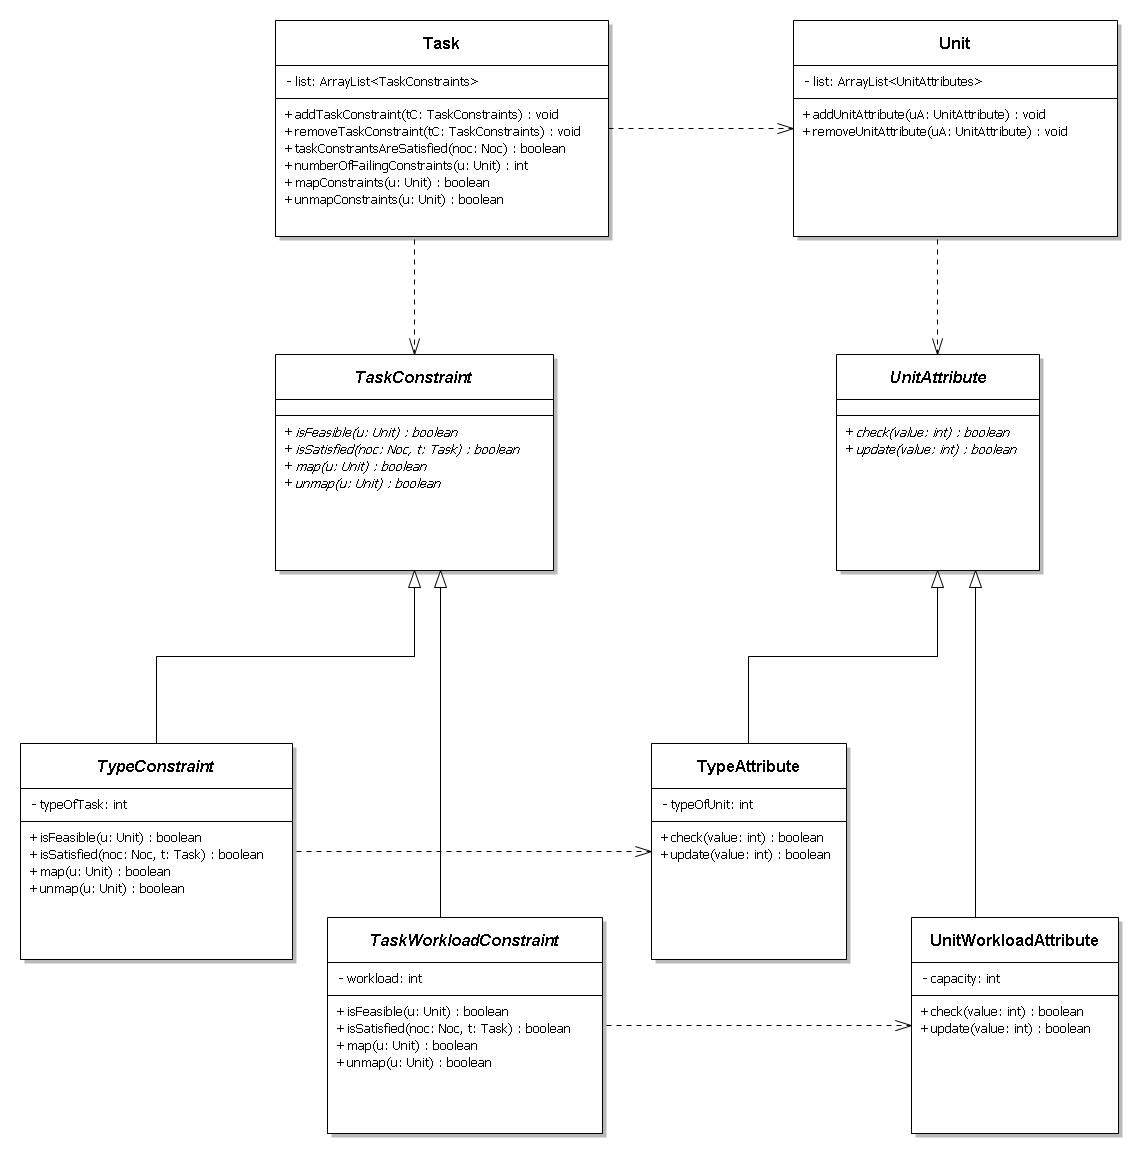
\includegraphics[width = 150mm]{bilder/task-unit.jpg}
  \caption{Klassendiagramm zum Lösen von Bindungsanforderungen}\label{fig:klBind}
\end{figure}

\subsection{Routinganforderungen}\label{routinganforderung}

Das Klassendiagramm zum Lösen von Routinganforderungen (siehe Abbildung \ref{fig:klRoute}) ist dem von Bindungsanforderungen sehr ähnlich. So sind die Methoden und deren Funktionalitäten gleich. Der Unterschied zu den Bindungsanforderungen besteht darin, dass nicht wie bei den Bindungsanforderungen die Attribute von nur einer Kachel (Unit) überprüft bzw. aktualisiert werden. Bei den Routinganforderungen werden die Attribute von mehreren Links, die zuvor mithilfe eines Routingalgorithmuses ermittelt  wurden, nachgeprüft oder erneuert. \\
\\
Die Routinganforderung MaxHopConstraint ist ein Spezialfall. Diese Anforderung benötigt kein LinkAttribut wie z. B. BandwidthConstraint, da sie nur überprüft, ob die Anzahl der Links in der zuvor berechneten Route eine maximal Zahl (maxHops) nicht überschritten wird.
\begin{figure}[H]\centering
  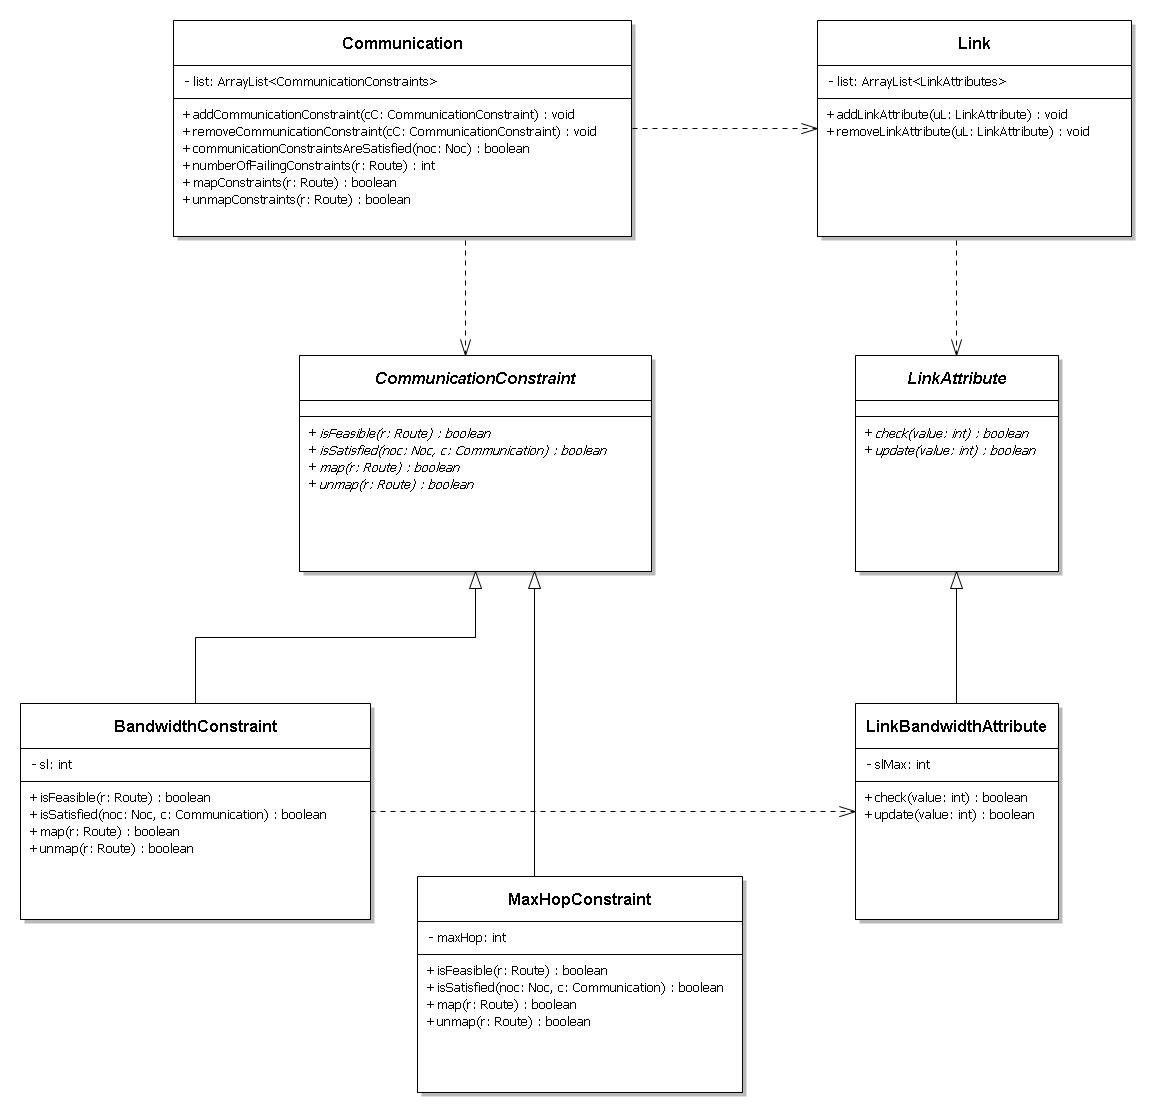
\includegraphics[width = 150mm]{bilder/communication-link.jpg}
  \caption{Klassendiagramm zum Lösen von Routinganforderungen}\label{fig:klRoute}
\end{figure}

\subsection{Hinzufügen von Anforderungen}
Um Anforderungen hinzuzufügen, wird in der Klasse Task bzw. Communication die Funktion addTaskConstraint bzw. addCommunicationConstraint aufgerufen. Die Anforderung wir in der ArrayListe list gespeichert. Falls eine Anforderung vom gleiche Typ schon vorhanden ist, wird diese durch die neue Anforderung ersetzt. Jede Anforderung (außer der MaxHopsConstraint) benötigt ein Unit- oder LinkAttribute, die beim Konfigurieren des NoCs schon mit addUnitAttribute bzw. addLinkAttribute hinzugefügt werden müssen.

\subsection{Überprüfen von Anforderungen}
Um zu überprüfen, ob alle Bindungsanforderungen erfüllt sind, wird in der Klasse Task die Methode taskConstraintsAreSatisfied aufgerufen. Diese Funktion ruft bei jedem Listeneintrag die Funktion isSatisfied. isSatisfied überprüft, ob der Task schon auf eine Kachel des Network-on-Chips eingebettet wurde und ob das dazugehörige UnitAttribute einen Fehler meldet.\\
\\
Mit der Funktion numberOfFailingConstraints in der Klasse Task kann man herausfinden, wie viele Bindungsanforderungen missachtet werden, wenn der Task zu einer Kachel zugeordnet wird. Hierzu wird für jeden Listeneintrag die isFeasible-Methode aufgerufen.\\
\\
Die Überprüfung der Routinganforderungen funktionieren nach dem gleichen Schemata.

\subsection{Zuordnen  von Anforderungen}
Wenn man die Funktion mapConstraints in der Klasse Task aufruft, werden alle für alle Listenelemente die Funktion map aufgerufen. Diese rufen, die Funktion update mit dem Übergabewert der Objektvariable des Listenelements vom dazugehörigen Attribut auf. Dadurch wird die Objektvariable des Attributs aktualisiert.\\
\\
Wenn man wieder die Anforderungen entziehen möchte, ruft man unmapConstraints auf. In dieser Funktion rufen alle Listenelemente unmap auf. Unmap ruft die Funktion update  des dazugehörigen Attriubtes auf. Diesmal ist der Übergabewert die negierte Objektvariable des Listenelements.